\documentclass{standalone}
\usepackage{tikz}
\usetikzlibrary{patterns, positioning}
\usepackage[sfdefault]{ClearSans} %% option 'sfdefault' activates Clear Sans as the default text font
\usepackage[T1]{fontenc}

\begin{document}
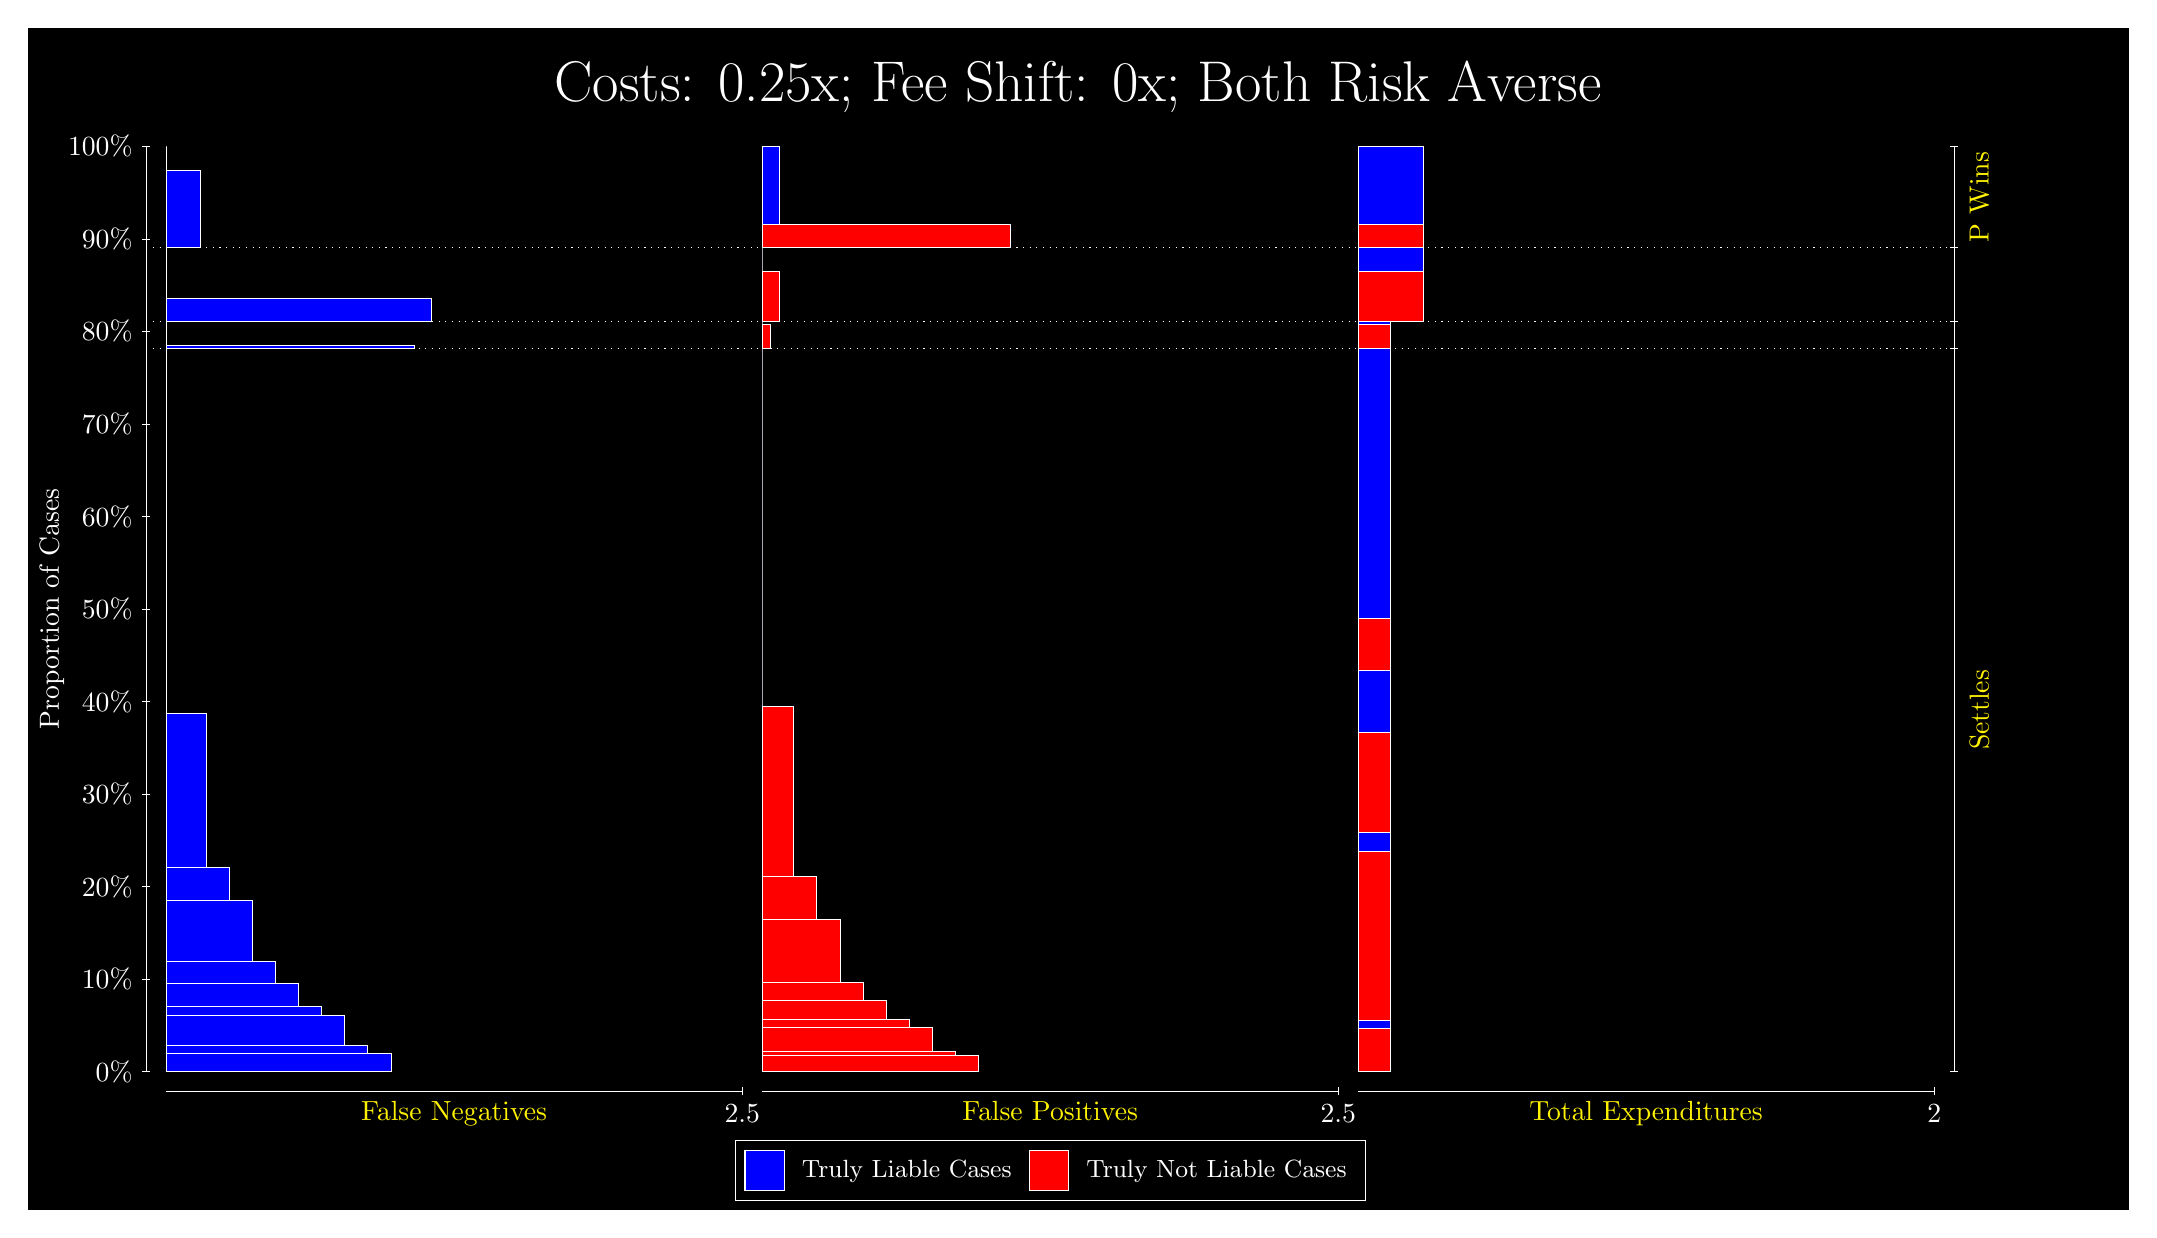
\begin{tikzpicture}
\draw[fill=black] (0,0) rectangle (26.667,15);
\draw[text=white] (0,13.5) rectangle (26.667,15) node[midway] {\huge Costs: 0.25x; Fee Shift: 0x; Both Risk Averse};
\draw[white, very thin] (1.5,1.75) -- (1.5,13.5);
\node[rotate=90, text=white, anchor=center] at (0.3, 7.625) {Proportion of Cases};
\draw[white, very thin] (1.45,1.75) -- (1.55,1.75);
\node[text=white, anchor=east] at (1.45, 1.75) {0\%};
\draw[white, very thin] (1.45,2.925) -- (1.55,2.925);
\node[text=white, anchor=east] at (1.45, 2.925) {10\%};
\draw[white, very thin] (1.45,4.1) -- (1.55,4.1);
\node[text=white, anchor=east] at (1.45, 4.1) {20\%};
\draw[white, very thin] (1.45,5.275) -- (1.55,5.275);
\node[text=white, anchor=east] at (1.45, 5.275) {30\%};
\draw[white, very thin] (1.45,6.45) -- (1.55,6.45);
\node[text=white, anchor=east] at (1.45, 6.45) {40\%};
\draw[white, very thin] (1.45,7.625) -- (1.55,7.625);
\node[text=white, anchor=east] at (1.45, 7.625) {50\%};
\draw[white, very thin] (1.45,8.8) -- (1.55,8.8);
\node[text=white, anchor=east] at (1.45, 8.8) {60\%};
\draw[white, very thin] (1.45,9.975) -- (1.55,9.975);
\node[text=white, anchor=east] at (1.45, 9.975) {70\%};
\draw[white, very thin] (1.45,11.15) -- (1.55,11.15);
\node[text=white, anchor=east] at (1.45, 11.15) {80\%};
\draw[white, very thin] (1.45,12.325) -- (1.55,12.325);
\node[text=white, anchor=east] at (1.45, 12.325) {90\%};
\draw[white, very thin] (1.45,13.5) -- (1.55,13.5);
\node[text=white, anchor=east] at (1.45, 13.5) {100\%};

\draw[white, very thin] (24.457,1.75) -- (24.457,13.5);
\draw[white, very thin] (24.407,1.75) -- (24.507,1.75);
\node[anchor=west] at (24.407, 1.75) {};
\draw[white, very thin] (24.407,10.936) -- (24.507,10.936);
\node[anchor=west] at (24.407, 10.936) {};
\draw[white, very thin] (24.407,11.273) -- (24.507,11.273);
\node[anchor=west] at (24.407, 11.273) {};
\draw[white, very thin] (24.407,12.212) -- (24.507,12.212);
\node[anchor=west] at (24.407, 12.212) {};
\draw[white, very thin] (24.407,13.5) -- (24.507,13.5);
\node[anchor=west] at (24.407, 13.5) {};

\draw[white, very thin, fill=blue] (1.75,1.75) rectangle (4.6044,1.9826);
\draw[white, very thin, fill=blue] (1.75,1.9826) rectangle (4.3116,2.0828);
\draw[white, very thin, fill=blue] (1.75,2.0828) rectangle (4.0188,2.4686);
\draw[white, very thin, fill=blue] (1.75,2.4686) rectangle (3.7261,2.5795);
\draw[white, very thin, fill=blue] (1.75,2.5795) rectangle (3.4333,2.8756);
\draw[white, very thin, fill=blue] (1.75,2.8756) rectangle (3.1406,3.1493);
\draw[white, very thin, fill=blue] (1.75,3.1493) rectangle (2.8478,3.9209);
\draw[white, very thin, fill=blue] (1.75,3.9209) rectangle (2.5551,4.3421);
\draw[white, very thin, fill=blue] (1.75,4.3421) rectangle (2.2623,6.3012);
\draw[white, very thin, fill=red] (1.75,6.3012) rectangle (1.75,10.936);
\draw[white, very thin, fill=blue] (1.75,10.936) rectangle (4.8971,10.973);
\draw[white, very thin, fill=red] (1.75,10.973) rectangle (1.75,11.273);
\draw[white, very thin, fill=blue] (1.75,11.273) rectangle (5.1167,11.574);
\draw[white, very thin, fill=red] (1.75,11.574) rectangle (1.75,12.212);
\draw[white, very thin, fill=blue] (1.75,12.212) rectangle (2.1891,13.197);
\draw[white, very thin, fill=red] (1.75,13.197) rectangle (1.75,13.5);
\draw[white, very thin, fill=red] (9.3189,1.75) rectangle (12.063,1.96);
\draw[white, very thin, fill=red] (9.3189,1.96) rectangle (11.771,2.0125);
\draw[white, very thin, fill=red] (9.3189,2.0125) rectangle (11.478,2.3057);
\draw[white, very thin, fill=red] (9.3189,2.3057) rectangle (11.185,2.4089);
\draw[white, very thin, fill=red] (9.3189,2.4089) rectangle (10.892,2.649);
\draw[white, very thin, fill=red] (9.3189,2.649) rectangle (10.6,2.8812);
\draw[white, very thin, fill=red] (9.3189,2.8812) rectangle (10.307,3.6825);
\draw[white, very thin, fill=red] (9.3189,3.6825) rectangle (10.014,4.2349);
\draw[white, very thin, fill=red] (9.3189,4.2349) rectangle (9.7214,6.3847);
\draw[white, very thin, fill=blue] (9.3189,6.3847) rectangle (9.3189,10.936);
\draw[white, very thin, fill=red] (9.3189,10.936) rectangle (9.4287,11.236);
\draw[white, very thin, fill=blue] (9.3189,11.236) rectangle (9.3189,11.273);
\draw[white, very thin, fill=red] (9.3189,11.273) rectangle (9.5384,11.911);
\draw[white, very thin, fill=blue] (9.3189,11.911) rectangle (9.3189,12.212);
\draw[white, very thin, fill=red] (9.3189,12.212) rectangle (12.466,12.515);
\draw[white, very thin, fill=blue] (9.3189,12.515) rectangle (9.5384,13.5);
\draw[white, very thin, fill=red] (16.888,1.75) rectangle (17.299,2.3023);
\draw[white, very thin, fill=blue] (16.888,2.3023) rectangle (17.299,2.4025);
\draw[white, very thin, fill=red] (16.888,2.4025) rectangle (17.299,4.5524);
\draw[white, very thin, fill=blue] (16.888,4.5524) rectangle (17.299,4.785);
\draw[white, very thin, fill=red] (16.888,4.785) rectangle (17.299,6.0586);
\draw[white, very thin, fill=blue] (16.888,6.0586) rectangle (17.299,6.8514);
\draw[white, very thin, fill=red] (16.888,6.8514) rectangle (17.299,7.5103);
\draw[white, very thin, fill=blue] (16.888,7.5103) rectangle (17.299,10.936);
\draw[white, very thin, fill=red] (16.888,10.936) rectangle (17.299,11.236);
\draw[white, very thin, fill=blue] (16.888,11.236) rectangle (17.299,11.273);
\draw[white, very thin, fill=red] (16.888,11.273) rectangle (17.711,11.911);
\draw[white, very thin, fill=blue] (16.888,11.911) rectangle (17.711,12.212);
\draw[white, very thin, fill=red] (16.888,12.212) rectangle (17.711,12.515);
\draw[white, very thin, fill=blue] (16.888,12.515) rectangle (17.711,13.5);
\draw[white, dotted] (1.5,10.936) -- (24.457,10.936);
\draw[white, dotted] (1.5,11.273) -- (24.457,11.273);
\draw[white, dotted] (1.5,12.212) -- (24.457,12.212);
\draw[white, very thin] (1.75,1.5) -- (9.0689,1.5);
\node[text=yellow, anchor=north] at (5.4094, 1.5) {False Negatives};
\draw[white, very thin] (9.0689,1.45) -- (9.0689,1.55);
\node[text=white, anchor=north] at (9.0689, 1.45) {2.5};

\draw[white, very thin] (9.3189,1.5) -- (16.638,1.5);
\node[text=yellow, anchor=north] at (12.978, 1.5) {False Positives};
\draw[white, very thin] (16.638,1.45) -- (16.638,1.55);
\node[text=white, anchor=north] at (16.638, 1.45) {2.5};

\draw[white, very thin] (16.888,1.5) -- (24.207,1.5);
\node[text=yellow, anchor=north] at (20.547, 1.5) {Total Expenditures};
\draw[white, very thin] (24.207,1.45) -- (24.207,1.55);
\node[text=white, anchor=north] at (24.207, 1.45) {2};

\node[text=yellow, centered, rotate=90] at (24.777, 6.3429) {Settles};


\node[text=yellow, centered, rotate=90] at (24.777, 12.856) {P Wins};

\draw (12.978300999999998,1.5) node[draw=none] (baseCoordinate) {};
\begin{scope}[align=center]
        \matrix[scale=0.5, draw=white, below=0.5cm of baseCoordinate, nodes={draw}, column sep=0.1cm]{
            \node[rectangle, draw, minimum width=0.5cm, minimum height=0.5cm, fill=blue] {}; &
            \node[draw=none, font=\small, text=white] (B) {Truly Liable Cases}; &
            \node[rectangle, draw, minimum width=0.5cm, minimum height=0.5cm, fill=red] {}; &
            \node[draw=none, font=\small, text=white] (B) {Truly Not Liable Cases}; \\
            };
\end{scope}

\end{tikzpicture}
\end{document}